Quando se trata de normas em sistemas multiagentes é de crucial importância definir claramente este termo. Isso se deve ao fato de que há diversos estudos que tratam o conceito de norma sobre perspectivas diferentes. Por exemplo, os estudos \cite{formalizeagent,formalizeagent2} apresentam normas, em sistemas multiagentes, para representar a presença de sociedades, institutos e organizações. 

Há estudos que tratam normas como maneiras dos agentes trabalharem de forma coordenada com propósito de cumprir um objetivo global e também como uma maneira de obedecer as autoridades do sistema \cite{modelingnormsforautnomousagent,amodelmultiagentsystemdynamicrelationship}. 

No \textit{MOISE+} normas são tratadas sob a ótica da lógica deôntica e é usada para especificar os agentes com dado papel no que condiz com as suas obrigações em relação as missões \cite{moiseframework,moiseframeworktwo}.

O estudo de \cite{dastaniframework} apresenta uma linguagem formal para especificar sistemas multiagentes normativos. Esta linguagem contém os conceitos de normas que são os mesmos usados neste texto. A Figura \ref{descreveprograma} apresenta a linguagem em notação EBNF \cite{dastaniframework}.

\begin{figure}[H]
  \centering
  \caption{Linguagem para descrever um programa de multiagentes normativos com a possibilidade de violações e sanções na notação EBNF segundo o texto \cite{dastaniframework}. Nesta notação, $<ident>$ é usado para denotar uma \textit{string} e $<int>$ inteiros. Os termos $<b-prop>$ e $<i-prop>$ são usados para designar dois tipos de conjuntos de proposições que são disjuntos entre si}
  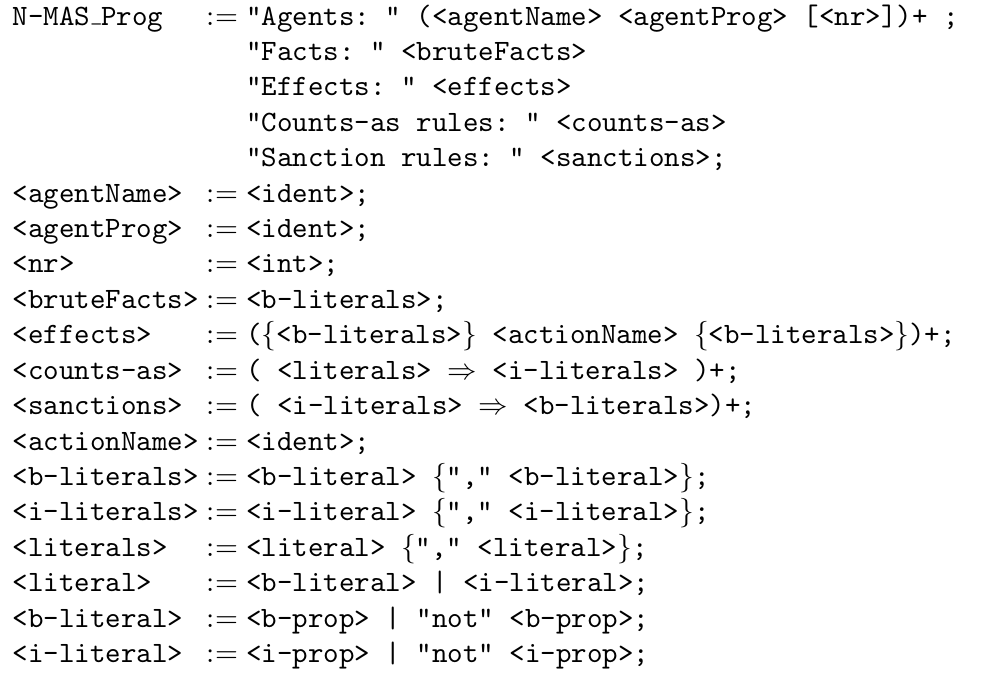
\includegraphics[width=0.8\linewidth]{figure/masprogram.png}
  \begin{center}
  	\cite{dastaniframework}
  \end{center} 
  \label{descreveprograma}
\end{figure}

Os \textit{Facts} implementados em forma de \textit{brute facts} definem os estados iniciais do sistema dentro de um ambiente compartilhado por todos os agentes. O termo \textit{Effects}, implementado por meio de $effects$ define como se dá a transição de estados do sistema. A tag $<actionName>$ representa os eventos que geram transição dos estados. Portanto uma norma é definida em termos de \textit{Counts\_as rules}. O termo $<counts-as>$ aponta para transição entre $<literals>$ e $<i-literals>$ representando os fatos que resultam em violações. Assim sendo em \cite{dastaniframework} as normas são descritas por intermédio de suas violações. Violação, dentro deste contexto, é dado como o descumprimento da norma \cite{ontologynormative}.

O termo \textit{Sanction Rules} aponta para $<sanctions>$ e esses, por sua vez, para a transição entre $<i-literals>$ e $<b-literals>$ sendo que esses $<i-literals>$ através de \textit{Counts\_as Rules}. Assim sendo, \textit{Sanction Rules} define as consequências da violação. Essas consequências denotam caráter negativo ao agente tendo como foco uma natureza de ordem punitiva.

A Figura \ref{exemploprograma} apresenta um programa escrito nesta linguagem. 

\begin{figure}[H]
  \centering
  \caption{Um programa descrito na linguagem proposta neste estudo onde um agente representa um passageiro em uma estação de trem que pode entrar com ou sem um \textit{ticket} na plataforma e no trem .}
  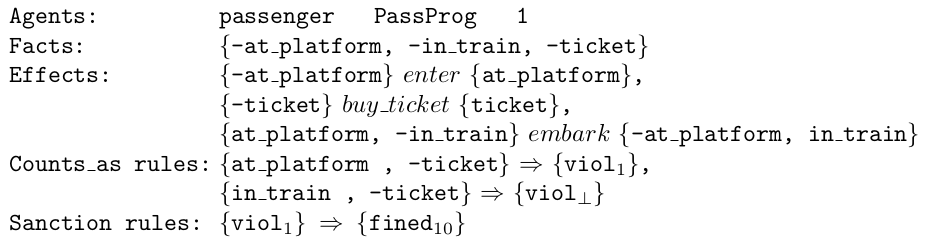
\includegraphics[width=0.8\linewidth]{figure/programdastani.png} 
  \begin{center}
  	\cite{dastaniframework}
  \end{center}
  \label{exemploprograma}
\end{figure}

Este programa contém um agente chamado de \textit{passenger} (especificações deste agente são detalhadas com maior rigor em \textit{PassProg}). Os \textit{Facts} deste programa são \textit{-at\_plataform} (agente não está na plataforma), \textit{-in\_train} (agente não está no trem) e \textit{-in\_ticket} (agente não possui o \textit{-in\_ticket}). As regras de \textit{Effects} apresentam dois $<actionName>$. O primeiro é denominado por \textit{enter} que tem por finalidade alternar entre os estados \textit{-at\_plataform} e \textit{at\_plataform}, 
ou seja, é uma ação onde o agente muda o estado de, não está na plataforma para, está na plataforma. O segundo estado é o \textit{buy\_ticket} que gera a transição entre os fatos \textit{-ticket} para \textit{ticket}, ou seja, na ocorrência \textit{buy\_ticket} o agente passa a ter um \textit{ticket} \cite{dastaniframework}.

O programa especifica duas regras em \textit{Counts\_as rules}. A primeira regra denota a ocorrência de uma violação para um agente que entra numa plataforma sem um \textit{ticket}. A segunda regra define que uma violação que acontece para o caso de um agente entrar em um trem sem um \textit{ticket} \cite{dastaniframework}.

O programa também define uma regra para \textit{Sanction rules}. Essa regra se aplica a $viol_1$, que - se verdade - então resulta no fato $fined_{10}$, cuja semântica denota um pagamento no valor de 10 unidades de moeda \cite{dastaniframework}.  